\section{Blockchain Integration and Decentralized Coordination}

The integration of Trusted Execution Environment technology with blockchain infrastructure addresses the fundamental coordination challenges inherent in decentralized artificial intelligence networks. While TEEs provide verifiable computation through hardware-based attestation, blockchain systems offer transparent registries, immutable audit trails, and economic incentive mechanisms that coordinate behavior among distributed participants. The combination of these technologies creates a comprehensive trust framework where cryptographic proofs from TEEs establish computational integrity while blockchain smart contracts enforce rules and manage state without centralized authorities. This section examines the architectural patterns, economic mechanisms, and technical implementations that enable effective blockchain integration for TEE-based AI systems.

The role of blockchain in decentralized AI extends beyond simple record-keeping to encompass multiple critical functions. Smart contracts implement registries that maintain authoritative records of approved models, their expected attestation measurements, and authorized deployment configurations. These registries enable discovery where clients can locate available models and retrieve the attestation policies necessary for verification. Enclave verification contracts validate attestation documents submitted by node operators and maintain lists of currently active nodes with valid attestations. Payment and settlement contracts coordinate financial transactions between service consumers and providers, holding funds in escrow and releasing payment upon cryptographic proof of service delivery. Governance contracts enable decentralized decision-making about protocol parameters, security policies, and network evolution through token-weighted voting mechanisms.

The gas cost economics of blockchain interactions represent a critical constraint that shapes integration architectures. Every operation executed by smart contracts on public blockchain networks consumes gas, a measure of computational resources with associated monetary costs that vary based on network congestion and cryptocurrency prices \cite{gas_optimization}. Naive implementations that perform expensive operations like ECDSA signature verification or certificate chain validation entirely on-chain can incur gas costs exceeding hundreds of dollars per transaction, rendering such approaches economically infeasible for frequent attestation verification. Practical blockchain integration requires careful optimization through hybrid architectures that perform expensive computations off-chain while committing minimal verification data on-chain, leveraging cryptographic commitments and fraud proofs to maintain security properties despite reduced on-chain computation.

\subsection{Smart Contract Architecture for Model and Enclave Registries}

The model registry smart contract serves as the foundational component for coordinating decentralized AI networks by maintaining authoritative records of available models and their security requirements. The registry stores model metadata including human-readable names, version identifiers, descriptions of model capabilities, and pointers to encrypted model artifacts in distributed storage systems. More critically, the registry records the expected Platform Configuration Register values that valid enclaves must exhibit when running each model. These PCR expectations enable clients and verifiers to determine whether an enclave claiming to execute a particular model actually contains the authorized code rather than a modified or substituted implementation.

The model registration process begins when model providers submit transactions to the registry contract containing model metadata and PCR values. The contract validates that the submitting address has appropriate permissions, either through ownership checks against model identifiers or through role-based access control where designated registrar addresses can add entries. Upon successful validation, the contract creates a new registry entry indexed by a unique model identifier computed as the hash of the model name and version. This content-addressed approach ensures that each distinct model version receives a unique identifier that cannot collide with other models. The contract emits events announcing the registration that observers can monitor to maintain synchronized local caches of registry contents.

The expected PCR values stored in the registry enable automated attestation verification by providing reference measurements against which actual enclave attestations can be compared. A typical registry entry includes PCR0 representing the complete enclave image hash, PCR1 measuring the kernel and boot infrastructure, and PCR2 capturing the application code including the specific inference implementation. Optional inclusion of PCR8 enables enforcement of signing requirements where only enclave images signed by authorized parties can validly execute the model. The registry may store multiple sets of PCR values for a single model to support different deployment configurations such as various optimization levels or compatibility with different infrastructure platforms.

The model authorization mechanisms within the registry contract implement access control over who can deploy and use registered models. Public models may be freely deployed by any node operator and used by any client without restrictions. Private models enforce access controls where only authorized addresses can deploy enclaves or submit inference requests. The contract implements authorization through allowlists maintained in contract storage that map model identifiers to sets of authorized addresses. Model providers can update these allowlists through contract functions that verify the caller's authority before modifying access permissions. This flexibility enables business models ranging from fully open source models to proprietary models with selective licensing.

The enclave registry contract complements the model registry by tracking which node operators currently have valid attestations proving they are running authorized enclave configurations. Node operators submit attestation documents to the registry along with metadata including network endpoints, capacity information, and pricing parameters. The contract performs validation of attestation documents through verification steps that check signatures, validate certificate chains against known root certificates, and compare PCR values against expected measurements from the model registry. Successfully verified enclaves are added to the active node registry with timestamps recording when verification occurred.

The enclave verification process within smart contracts must balance security thoroughness against gas cost constraints. Full verification including ECDSA signature validation, certificate chain traversal, and cryptographic hash computations can consume 80,000 to 100,000 gas units, translating to several dollars per verification at typical Ethereum gas prices \cite{ethereum_yellow}. This cost structure makes on-chain verification economically prohibitive for frequent attestation updates across large node fleets. Practical implementations employ off-chain verification where specialized verifier nodes perform complete attestation validation and submit only compact proofs of verification to on-chain contracts.

The off-chain verification architecture introduces verifier nodes that operate as trusted but verifiable intermediaries between enclave operators and blockchain contracts. Verifiers receive attestation documents from enclaves, perform complete cryptographic verification including signature validation and certificate chain checking, and submit verification results to the registry contract. The contract trusts the verifier's determination but implements accountability mechanisms including staking requirements where verifiers must lock collateral that can be slashed if they approve invalid attestations, challenge periods where other parties can dispute verification results by providing contradictory evidence, and fraud proofs that demonstrate verifier misbehavior through cryptographic evidence. This architecture reduces per-verification gas costs to 5,000 to 10,000 units while maintaining security through economic incentives and cryptographic accountability.

The registry expiration and renewal mechanisms address the three-hour certificate validity period inherent in AWS Nitro Enclaves attestation \cite{nitro_security}. Registry entries include timestamps indicating when verification occurred and validity periods beyond which the registration becomes stale. Clients querying the registry for active nodes filter out entries with expired timestamps to ensure they only interact with currently verified enclaves. Node operators must periodically refresh their registrations by submitting new attestation documents before expiration. The contract implements grace periods where registrations approaching expiration receive warnings but remain active, enabling smooth renewal without service disruptions from timing precision requirements.

\subsection{Inference Market and Payment Coordination}

The inference market smart contract coordinates economic interactions between clients requesting AI inference services and node operators providing those services through verified enclaves. The market implements a complete lifecycle spanning request submission, node assignment, service delivery verification, and payment settlement. This coordination occurs trustlessly without requiring participants to have pre-existing relationships or trust in intermediaries, relying instead on cryptographic proofs and economic guarantees enforced by the smart contract.

The request submission process begins when clients create transactions containing inference request metadata and payment. The metadata specifies the desired model identifier, priority or quality of service parameters, and deadline by which results must be delivered. The payment amount is locked in the contract's escrow where it remains inaccessible to both client and node operator until the request resolution conditions are met. The contract validates that the requested model exists in the model registry, that sufficient payment has been provided based on the model's pricing parameters, and that the client's address has appropriate authorization if the model enforces access controls.

The node selection algorithm implemented within the contract or through off-chain computation determines which registered enclave will service each request. Simple selection strategies include round-robin distribution across active nodes, random selection weighted by node capacity or stake, or price-based assignment where nodes bid for requests. More sophisticated selection considers node specialization where certain nodes may have optimized configurations for particular model types, geographic distribution to minimize latency between clients and assigned nodes, or reputation scores derived from historical performance. The selection logic must operate within gas constraints, potentially requiring off-chain computation of assignments with on-chain commitment to assignments through Merkle root publication.

The service delivery phase occurs off-chain through direct communication between clients and assigned enclaves. The client encrypts the actual inference input data using the enclave's public key obtained from its attestation document, ensuring confidentiality even though the parent instance proxies communication. The enclave performs inference, generates results, and creates cryptographic proof of correct execution. This proof may take various forms depending on the verification requirements, including attestation documents binding the computation to specific requests through nonce or user data fields, zero-knowledge proofs demonstrating correct computation without revealing model internals, or simply signed responses where the enclave's attestation provides evidence of code integrity.

The result submission and payment release phase brings the interaction back on-chain for settlement. The node operator submits proof of service delivery to the market contract along with any required cryptographic evidence. The contract verifies the proof, which may involve checking signatures, validating nonce correspondence, or confirming zero-knowledge proof validity. If verification succeeds and the submission occurs within the deadline, the contract releases payment from escrow to the node operator's address. If verification fails or the deadline expires, the contract returns payment to the client and may impose penalties on the assigned node through reputation decrements or stake slashing.

The dispute resolution mechanisms address scenarios where clients and node operators disagree about service delivery quality or correctness. Clients who believe they received incorrect results can initiate disputes by submitting evidence of misbehavior. The contract evaluates this evidence, potentially involving arbitration by designated resolver addresses or voting by token holders in decentralized governance. Successful disputes result in payment reversal and penalties against the node operator, while unsuccessful disputes may penalize the client for frivolous complaints. The economic incentives are structured to discourage baseless disputes while ensuring clients have recourse against genuinely faulty service.

The pricing mechanism within the market can be implemented through various models depending on network governance preferences. Fixed pricing assigns costs per inference request based on model size, complexity, or provider preferences. Dynamic pricing adjusts costs based on supply and demand, increasing prices during high demand periods when capacity is constrained. Auction-based pricing allows nodes to bid for serving requests, with the lowest bidder winning assignment. The pricing model affects the economic efficiency of the network and the distribution of value between providers and consumers, making it a critical governance parameter.

\subsection{Gas Optimization Techniques and Hybrid Architectures}

The high cost of on-chain computation necessitates sophisticated optimization techniques that minimize gas consumption while preserving security properties. These optimizations exploit the asymmetry between expensive on-chain computation and cheap off-chain computation, committing to off-chain results through compact on-chain data structures that enable verification without repeating expensive operations. Understanding these techniques is essential for implementing economically viable blockchain integration at scale.

The Merkle tree commitment pattern represents a fundamental optimization for representing large datasets with compact on-chain footprints \cite{merkle_trees}. Rather than storing complete attestation documents on-chain, the contract stores only the Merkle root computed from attestation data. Verifiers can prove that specific attestations exist in the committed set by providing Merkle proofs consisting of the hash path from the attestation to the root. The on-chain verification operation hashes the provided data and path elements, comparing the result against the stored root. This verification requires only logarithmic space and computation in the size of the dataset, reducing gas costs from tens of thousands of units for full attestation storage to thousands of units for root storage and proof verification.

\begin{figure}[htbp]
\centering
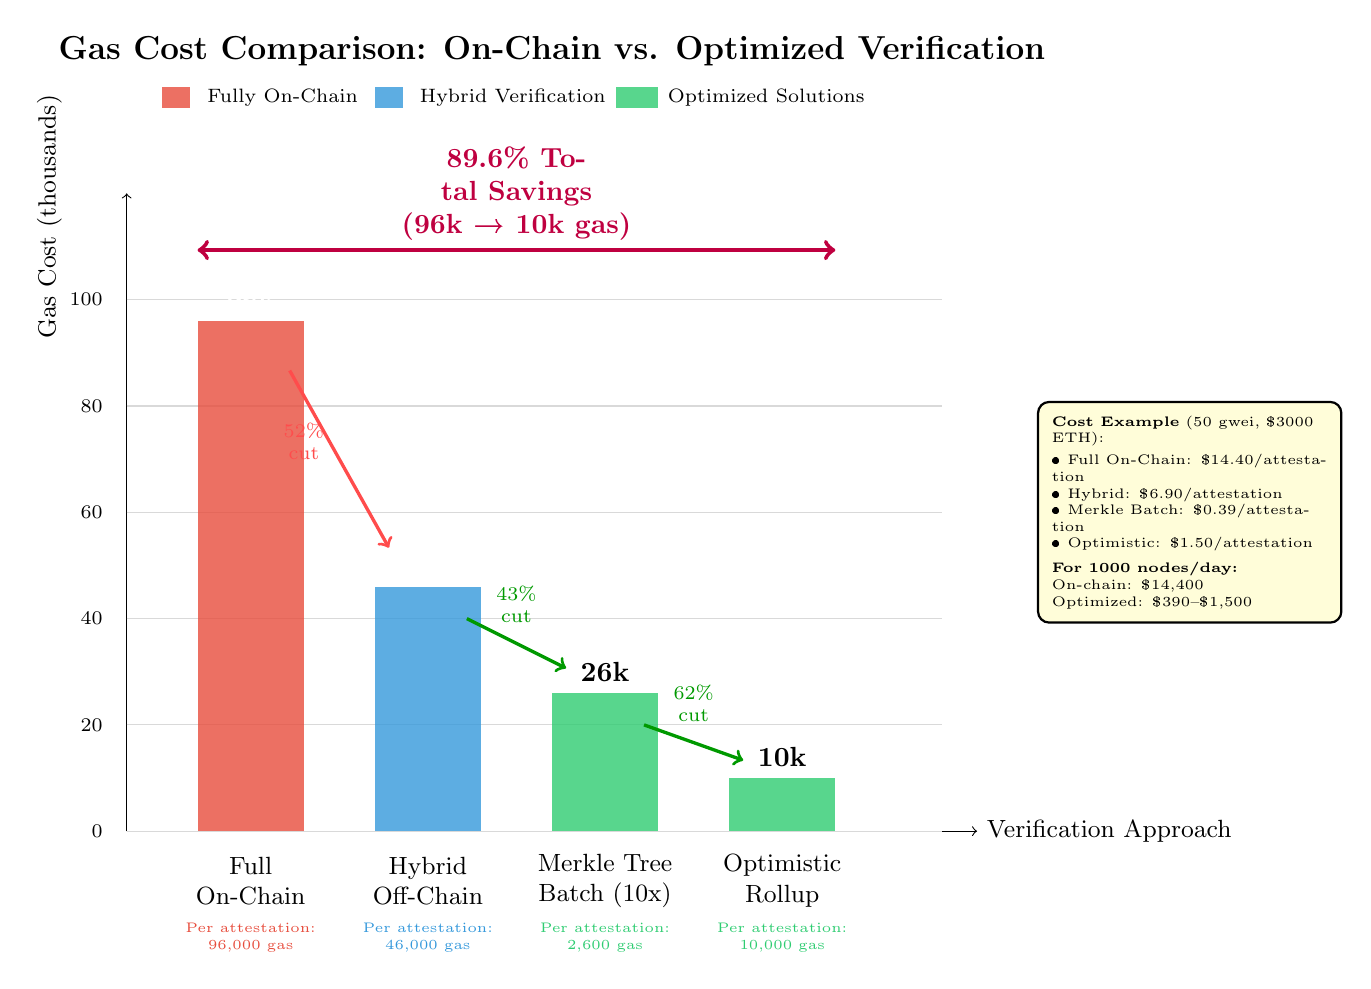
\begin{tikzpicture}[scale=0.9]
    % Title
    \node[font=\bfseries\large] at (6, 11) {Gas Cost Comparison: On-Chain vs. Optimized Verification};
    
    % Define colors
    \definecolor{onchaincolor}{RGB}{231, 76, 60}
    \definecolor{hybridcolor}{RGB}{52, 152, 219}
    \definecolor{optimizedcolor}{RGB}{46, 204, 113}
    
    % Y-axis
    \draw[->] (0, 0) -- (0, 9) node[anchor=south, rotate=90, yshift=0.7cm, xshift=-0.3cm, font=\small] {Gas Cost (thousands)};
    \draw[->] (0, 0) -- (12, 0) node[anchor=west, font=\small] {Verification Approach};
    
    % Y-axis scale
    \foreach \y/\label in {0/0, 1.5/20, 3/40, 4.5/60, 6/80, 7.5/100} {
        \draw[gray!30, thin] (0, \y) -- (11.5, \y);
        \node[anchor=east, font=\scriptsize] at (-0.2, \y) {\label};
    }
    
    % Bar 1: Full On-Chain Verification (96k = 7.2 on scale)
    \fill[onchaincolor, opacity=0.8] (1, 0) rectangle (2.5, 7.2);
    \node[font=\small, text width=2cm, align=center] at (1.75, -0.7) {Full\\On-Chain};
    \node[font=\small, white, font=\bfseries] at (1.75, 7.5) {96k};
    
    % Bar 2: Hybrid Approach (46k = 3.45 on scale)
    \fill[hybridcolor, opacity=0.8] (3.5, 0) rectangle (5, 3.45);
    \node[font=\small, text width=2cm, align=center] at (4.25, -0.7) {Hybrid\\Off-Chain};
    \node[font=\small, white, font=\bfseries] at (4.25, 3.75) {46k};
    
    % Bar 3: Merkle Tree Batch (26k = 1.95 on scale)
    \fill[optimizedcolor, opacity=0.8] (6, 0) rectangle (7.5, 1.95);
    \node[font=\small, text width=2.5cm, align=center] at (6.75, -0.7) {Merkle Tree\\Batch (10x)};
    \node[font=\small, font=\bfseries] at (6.75, 2.25) {26k};
    
    % Bar 4: Optimistic Rollup (10k = 0.75 on scale)
    \fill[optimizedcolor, opacity=0.8] (8.5, 0) rectangle (10, 0.75);
    \node[font=\small, text width=2.5cm, align=center] at (9.25, -0.7) {Optimistic\\Rollup};
    \node[font=\small, font=\bfseries] at (9.25, 1.05) {10k};
    
    % Per-attestation costs below bars
    \node[font=\tiny, onchaincolor, text width=2.5cm, align=center] at (1.75, -1.5) {Per attestation:\\96,000 gas};
    \node[font=\tiny, hybridcolor, text width=2.5cm, align=center] at (4.25, -1.5) {Per attestation:\\46,000 gas};
    \node[font=\tiny, optimizedcolor, text width=2.5cm, align=center] at (6.75, -1.5) {Per attestation:\\2,600 gas};
    \node[font=\tiny, optimizedcolor, text width=2.5cm, align=center] at (9.25, -1.5) {Per attestation:\\10,000 gas};
    
    % Cost savings arrows - adjusted to not overlap
    \draw[->, very thick, red!70] (2.3, 6.5) -- (3.7, 4);
    \node[font=\scriptsize, red!70, text width=1.3cm, align=center] at (2.5, 5.5) {52\%\\cut};
    
    \draw[->, very thick, green!60!black] (4.8, 3) -- (6.2, 2.3);
    \node[font=\scriptsize, green!60!black, text width=1.3cm, align=center] at (5.5, 3.2) {43\%\\cut};
    
    \draw[->, very thick, green!60!black] (7.3, 1.5) -- (8.7, 1);
    \node[font=\scriptsize, green!60!black, text width=1.3cm, align=center] at (8, 1.8) {62\%\\cut};
    
    % Total savings annotation
    \draw[<->, ultra thick, purple] (1, 8.2) -- (10, 8.2);
    \node[font=\normalsize, purple, font=\bfseries, text width=3.5cm, align=center] at (5.5, 9) {89.6\% Total Savings\\(96k → 10k gas)};
    
    % Dollar cost example box - moved outside graph to the right
    \node[draw, thick, rounded corners, fill=yellow!15, text width=3.5cm, align=left, font=\tiny, inner sep=5pt] at (15, 4.5) {
        \textbf{Cost Example} (50 gwei, \$3000 ETH):\\[2pt]
        • Full On-Chain: \$14.40/attestation\\
        • Hybrid: \$6.90/attestation\\
        • Merkle Batch: \$0.39/attestation\\
        • Optimistic: \$1.50/attestation\\[3pt]
        \textbf{For 1000 nodes/day:}\\
        On-chain: \$14,400\\
        Optimized: \$390--\$1,500
    };
    
    % Legend - repositioned with proper spacing
    \fill[onchaincolor, opacity=0.8] (0.5, 10.2) rectangle (0.9, 10.5);
    \node[anchor=west, font=\scriptsize] at (1, 10.35) {Fully On-Chain};
    
    \fill[hybridcolor, opacity=0.8] (3.5, 10.2) rectangle (3.9, 10.5);
    \node[anchor=west, font=\scriptsize] at (4, 10.35) {Hybrid Verification};
    
    \fill[optimizedcolor, opacity=0.8] (7.5, 10.2) rectangle (6.9, 10.5);
    \node[anchor=west, font=\scriptsize] at (7.5, 10.35) {Optimized Solutions};
    
\end{tikzpicture}
\caption{Gas cost analysis for different attestation verification strategies on Ethereum. Hybrid architectures with off-chain verification and on-chain commitments reduce costs by 52\%, while Merkle tree batching achieves 97\% reduction. For large-scale deployments with thousands of nodes, optimized strategies are essential for economic viability.}
\label{fig:gas_optimization}
\end{figure}

The batching approach amortizes fixed transaction costs across multiple operations by grouping them into single transactions. Rather than submitting individual attestation verifications that each incur base transaction costs of 21,000 gas, a batch verification transaction combines multiple attestations into one submission \cite{gas_optimization}. The contract processes all attestations in a single execution context, amortizing the fixed costs and reducing the per-attestation cost. Batch processing can achieve 50 to 70 percent cost reduction compared to individual transactions when batch sizes reach dozens of operations. The trade-off involves delayed processing where attestations must accumulate before batch submission, potentially creating latency between enclave startup and registry activation.

The state compression techniques reduce storage costs by encoding information compactly rather than using straightforward but verbose representations. Platform Configuration Register values as 48-byte hashes consume substantial storage when hundreds or thousands of enclaves register. The contract can store only the most significant bytes of PCR values if uniqueness within the expected set is guaranteed, reducing storage to 8 or 16 bytes per PCR. Alternatively, contracts can store references to shared PCR sets where multiple enclaves exhibit identical measurements, eliminating redundant storage of common values. These compressions reduce storage costs but increase computational complexity during verification as decompression logic must execute to recover full values.

The optimistic verification pattern implements fraud-proof-based security where operations proceed under the assumption of correctness with challenges resolving disputes. When a verifier claims that an attestation is valid, the contract accepts this claim without on-chain verification but opens a challenge window during which other parties can dispute the verification. If a challenger provides cryptographic proof that the attestation is invalid, the original verifier's stake is slashed and redistributed to the challenger and the network. If no valid challenge emerges during the window, the verification is finalized. This pattern reduces normal-case gas costs dramatically since most verifications are honest and require no on-chain computation beyond accepting the verifier's claim and starting the challenge timer.

\begin{table}[htbp]
\centering
\caption{Gas Cost Analysis for On-Chain Attestation Verification Strategies}
\label{tab:gas-optimization}
\footnotesize
\begin{tabular}{@{}lrrrll@{}}
\toprule
\textbf{Strategy} & \textbf{Gas} & \textbf{USD*} & \textbf{Ops} & \textbf{Latency} & \textbf{Sec.} \\
\midrule
\multicolumn{6}{l}{\textit{\textbf{On-Chain Verification}}} \\
Full ECDSA & 96k & \$14.40 & 312 & Immediate & High \\
+ Cert Chain & 125k & \$18.75 & 240 & Immediate & High \\
+ 6 PCRs & 146k & \$21.90 & 205 & Immediate & High \\
Complete & 180k & \$27.00 & 166 & Immediate & High \\
\midrule
\multicolumn{6}{l}{\textit{\textbf{Hybrid Off-Chain}}} \\
Off-Chain + Commit & 46k & \$6.90 & 652 & 1-2 blk & High \\
+ Fraud Proof & 48k & \$7.20 & 625 & 10-20 blk & High \\
Verifier Sig & 42k & \$6.30 & 714 & 1 blk & Med \\
Multi-Verifier (3/5) & 58k & \$8.70 & 517 & 2-3 blk & V.High \\
\midrule
\multicolumn{6}{l}{\textit{\textbf{Merkle Batching}}} \\
Batch-10 (total) & 26k & \$3.90 & 1.1k & 5-10 blk & High \\
\quad per attest. & 2.6k & \$0.39 & --- & --- & --- \\
Batch-50 (total) & 85k & \$12.75 & 352 & 20-30 blk & High \\
\quad per attest. & 1.7k & \$0.26 & --- & --- & --- \\
Batch-100 (total) & 155k & \$23.25 & 193 & 40-60 blk & High \\
\quad per attest. & 1.6k & \$0.23 & --- & --- & --- \\
Merkle Proof & 12k & \$1.80 & 2.5k & Immediate & High \\
\midrule
\multicolumn{6}{l}{\textit{\textbf{Optimistic Patterns}}} \\
Optimistic Accept & 10k & \$1.50 & 3k & 1-7 days & Med \\
Challenge & 85k & \$12.75 & --- & Immediate & --- \\
Fraud Proof Exec & 120k & \$18.00 & --- & Immediate & --- \\
ZK-SNARK & 250k & \$37.50 & 120 & Immediate & High \\
\quad Gen (off-chain) & --- & \$2.50 & --- & 10-60s & --- \\
\midrule
\multicolumn{6}{l}{\textit{\textbf{State Compression}}} \\
PCR Hash (32B) & 22k & \$3.30 & 1.4k & Immediate & Med \\
Truncated (8B) & 12k & \$1.80 & 2.5k & Immediate & Low \\
Bloom Filter & 95k & \$14.25 & 315 & Immediate & Med \\
\midrule
\multicolumn{6}{l}{\textit{\textbf{Layer 2 Solutions}}} \\
Arbitrum & 8k & \$0.12 & --- & 1-2 blk & High \\
Optimism & 9.5k & \$0.14 & --- & 1-2 blk & High \\
Polygon zkEVM & 12k & \$0.08 & --- & 1 blk & High \\
StarkNet & 15k & \$0.05 & --- & 1-2 blk & High \\
\midrule
\multicolumn{6}{l}{\textit{\textbf{Production (1000 nodes/day)}}} \\
Full On-Chain & --- & \$27k & \multicolumn{3}{l}{\textbf{Cost Savings}} \\
Hybrid & --- & \$6.9k & \multicolumn{3}{l}{Hybrid: \textbf{74\%}} \\
Merkle-100 & --- & \$233 & \multicolumn{3}{l}{Merkle: \textbf{99.1\%}} \\
L2 Arbitrum & --- & \$120 & \multicolumn{3}{l}{Layer 2: \textbf{99.6\%}} \\
\bottomrule
\end{tabular}
\begin{tablenotes}
\scriptsize
\item * 50 gwei, \$3k ETH. k=thousands. Ops=ops/block (30M gas limit). Sec.=Security level.
\end{tablenotes}
\end{table}

The aggregation signature schemes enable compact representation of multiple signatures through cryptographic protocols that combine individual signatures into one compact proof \cite{threshold_crypto}. Rather than verifying dozens of ECDSA signatures on-chain for a set of attestations, the contract verifies a single aggregate signature that proves all individual signatures are valid. The BLS signature scheme supports efficient aggregation where multiple signatures can be combined into one signature of the same size as individual signatures, with verification complexity independent of the number of signers. Adopting aggregate signatures requires changes to the attestation signing process to use BLS rather than ECDSA, potentially conflicting with existing TEE attestation infrastructure that uses ECDSA on the P-384 curve.

The layer-two scaling approaches offload transaction processing to secondary networks that settle periodically to the main blockchain, reducing costs through batching and off-chain computation. Rollup technologies including optimistic rollups and zero-knowledge rollups process thousands of transactions off-chain, committing only compact state roots and proofs to the main chain \cite{ethereum_yellow}. Decentralized AI networks can deploy their attestation and payment contracts on layer-two networks, achieving costs reduced by factors of 10 to 100 compared to layer-one deployment. The trade-offs involve added complexity from interacting with layer-two infrastructure, potential security risks from the layer-two protocol itself, and delayed finality as layer-two state settles asynchronously to layer one.

The event-driven off-chain synchronization pattern minimizes on-chain storage by emitting events that off-chain observers process to maintain synchronized local state. Rather than storing complete attestation documents or model metadata in contract storage where each byte incurs permanent storage costs, the contract emits events containing this data during transactions. Clients and nodes subscribe to these events, maintaining local databases that mirror on-chain state. The contract stores only minimal data necessary for verification and dispute resolution, relying on event replay for state reconstruction if local databases are lost. This pattern reduces storage costs but creates dependencies on event logs remaining available and nodes maintaining proper synchronization.

\subsection{Economic Security and Incentive Mechanisms}

The economic security model of decentralized AI networks built on TEE attestation combines cryptographic proofs with financial incentives to align participant behavior with network objectives. While attestation provides technical verification that code is running correctly, economic mechanisms ensure that participants have strong incentives to maintain that correct behavior over time and to avoid actions that compromise network security or reliability. These mechanisms draw from established patterns in blockchain consensus and proof-of-stake systems adapted for the specific requirements of verifiable AI services \cite{stake_based_consensus}.

The staking requirement forms the foundation of economic security by requiring node operators to lock collateral before participating in the network. Minimum stake amounts measured in network tokens or stablecoins establish a financial commitment that operators forfeit if they violate protocol rules. The stake serves multiple purposes including creating costs for Sybil attacks where adversaries create many identities, providing collateral for slashing in response to misbehavior, and demonstrating long-term commitment to the network that aligns incentives with network health. Stake amounts must be calibrated to exceed the expected profit from attacks, ensuring rational actors find honest behavior more profitable than malicious actions.

The slashing mechanism punishes protocol violations by destroying or redistributing staked collateral when cryptographic evidence proves misbehavior. Slashable offenses include submitting invalid attestation documents where PCR values do not match registered expectations, failing to deliver inference results within promised deadlines, returning provably incorrect results when correct outputs can be determined, or attempting to extract model weights or user data through unauthorized means. The severity of slashing ranges from small percentage reductions for minor infractions to complete stake destruction for egregious violations. The cryptographic verifiability of attestation ensures that slashing can be triggered automatically by smart contracts when violations are proven, eliminating dependence on subjective human judgment.

The reward distribution system compensates honest participants for providing services and maintaining network security. Node operators earn fees from inference requests processed successfully, with payments flowing automatically through smart contract escrow. Additional rewards may be distributed from inflationary token issuance or network revenues to incentivize desired behaviors beyond basic service provision, such as maintaining high availability, participating in network governance, or running nodes in underserved geographic regions. The reward structure balances between providing sufficient incentives for participation and avoiding excessive token dilution or unsustainable treasury expenditures.

The reputation system complements cryptographic verification and economic incentives by tracking historical behavior and enabling participants to select counterparties based on past performance \cite{reputation_systems}. Reputation scores aggregate metrics including attestation renewal consistency, inference request completion rates, average response latency, and dispute frequency. High reputation nodes may command premium pricing or receive preferential assignment of requests. Low reputation nodes face reduced demand for their services, creating market-based incentives for maintaining service quality. Reputation systems must resist manipulation through Sybil attacks where adversaries create new identities to escape negative reputation, potentially requiring reputation transfer restrictions or aging requirements before new nodes can achieve high reputation.

The insurance mechanisms provide additional economic security by pooling risk across network participants. Node operators contribute premiums to insurance pools that compensate clients for losses from service failures or security breaches. The insurance creates alignment where operators have financial exposure to their actions beyond immediate transaction fees, incentivizing investment in security and reliability. Insurance pricing can reflect risk through higher premiums for nodes with lower attestation standards or poor historical performance. The collective nature of insurance creates peer pressure for maintaining network-wide security standards as all operators share exposure to systemic risks.

The governance token economics enable decentralized control over network parameters while creating value for stakeholders who invest in network success. Token holders vote on proposals affecting protocol rules, fee structures, slashing parameters, and security policies. The token value derives from rights to influence protocol evolution and potentially from cash flows through fee capture or stake-weighted reward distribution. This tokenization aligns long-term stakeholder interests with network health, as token value appreciation depends on the network providing valuable services with strong security properties.

\subsection{Multi-Chain Attestation and Cross-Chain Integration}

The deployment of TEE-based AI networks across multiple blockchain platforms addresses several strategic objectives including reducing centralization on any single blockchain, expanding addressable markets by reaching users across different ecosystems, and improving resilience through diversity in infrastructure dependencies. Multi-chain architectures introduce technical challenges in maintaining consistent state across chains, coordinating cross-chain payments, and preventing replay attacks where attestations or transactions intended for one chain are fraudulently reused on another.

The cross-chain attestation verification problem requires that attestation documents generated for one blockchain context remain verifiable on other chains without introducing security vulnerabilities. A naive approach of using identical attestation documents across chains creates replay attack opportunities where a valid attestation submitted on chain A could be copied and submitted on chain B by an unauthorized party. The solution involves binding attestations to specific chain contexts through inclusion of chain identifiers in the user data or nonce fields of attestation documents. The enclave generates distinct attestations for each chain it wishes to participate on, with the chain identifier cryptographically bound to the attestation through the hypervisor's signature.

The cross-chain state synchronization challenge arises from the need to maintain consistent views of model registries, enclave registrations, and other shared state across multiple blockchain networks that operate independently. A model registered on Ethereum should be discoverable by clients on Polygon or Binance Smart Chain without requiring duplicate registration transactions on each chain. Synchronization solutions include relay networks where specialized nodes observe state changes on one chain and submit corresponding transactions to other chains, maintaining eventual consistency across the multi-chain system. Merkle proofs enable efficient verification that state observed on one chain matches the canonical state on another chain without duplicating complete state on all chains.

The cross-chain payment and settlement mechanisms coordinate financial transactions that may involve assets on different blockchains. A client holding USDC on Polygon may wish to pay for inference services from a node operator accepting payments on Ethereum. Cross-chain payment solutions include bridge protocols that lock tokens on one chain while minting equivalent tokens on another chain, enabling value transfer across chains. Atomic swap protocols enable direct exchange of assets across chains without trusted intermediaries, using hash time-locked contracts that ensure both sides of the exchange complete or both fail. Layer-zero protocols implement unified messaging across chains, enabling smart contracts on one chain to trigger actions on other chains through verified message passing.

The oracle problem in cross-chain integration involves reliably communicating information from one blockchain to another in a trustless manner. While TEE attestation provides cryptographic evidence within a single chain context, proving to chain B that an attestation was verified on chain A requires trusted relays or cryptographic proofs of chain A state. Light client verification enables contracts on chain B to validate chain A block headers and transaction proofs, establishing trustless bridges at the cost of significant on-chain computation. Optimistic verification with fraud proofs reduces costs by assuming relayed information is correct unless challenged, with economic penalties discouraging false relays.

The multi-chain deployment strategies for decentralized AI networks range from symmetric deployments where equivalent infrastructure operates on each supported chain to hub-and-spoke architectures where one chain serves as the canonical source of truth with other chains synchronizing from it. Symmetric deployments maximize decentralization and resilience but incur higher maintenance costs from operating separate registry and market contracts on each chain. Hub-and-spoke architectures reduce complexity but create dependencies on the hub chain that could become bottlenecks or single points of failure. Hybrid approaches may maintain canonical model registries on a primary chain while supporting inference markets on multiple secondary chains that reference the primary registry.

The governance challenges in multi-chain networks involve coordinating decision-making across communities that may have different preferences or voting patterns. Protocol upgrades affecting attestation requirements or economic parameters should ideally be consistent across all supported chains to avoid fragmentation where different chains diverge in their security properties or service characteristics. Multi-chain governance solutions include synchronized voting where proposals must achieve approval on all chains before implementation, weighted voting where different chains contribute votes proportional to their activity or stake, or independent governance where each chain community makes autonomous decisions accepting potential divergence.

\subsection{Smart Contract Security and Audit Considerations}

The security of smart contracts implementing blockchain integration for TEE-based AI networks requires careful attention to common vulnerability patterns and thorough auditing procedures. Smart contract vulnerabilities can undermine the security guarantees provided by TEE attestation if contracts fail to properly validate inputs, handle edge cases, or resist economic attacks. The immutability of deployed contracts makes thorough security analysis essential before mainnet deployment, as vulnerabilities cannot be easily patched once discovered in production \cite{smart_contracts_security}.

The input validation requirements for attestation data are particularly critical because improper validation could allow invalid attestations to be accepted as genuine. Contracts must verify that attestation documents conform to expected CBOR structure, that signature lengths match algorithm requirements, that PCR maps contain valid indices and value sizes, and that timestamps fall within acceptable ranges. Insufficient validation could enable malformed attestations to bypass verification logic or cause contract failures through unexpected data formats. Fuzzing techniques that generate random or malformed inputs help identify validation gaps during testing.

The reentrancy vulnerabilities arise when contracts make external calls that could recursively invoke contract functions before the initial call completes, potentially violating state invariants. Payment distribution logic must follow checks-effects-interactions patterns where balance updates occur before external calls that could trigger reentrancy. The use of reentrancy guards that prevent recursive calls during sensitive operations provides additional protection. Modern Solidity compiler versions include reentrancy detection but cannot catch all patterns, necessitating manual review and explicit guard implementation.

The integer overflow and underflow protections prevent arithmetic errors that could corrupt contract state or enable unauthorized actions. Solidity 0.8 and later includes automatic overflow checking that reverts transactions when arithmetic exceeds type bounds, eliminating a major historical vulnerability class. However, contracts must still carefully consider edge cases in financial calculations where rounding errors could accumulate or where incentive formulas might produce unexpected results with extreme input values. Formal verification of arithmetic operations provides high assurance of correctness for security-critical computations.

The access control vulnerabilities occur when contract functions lack proper authorization checks, enabling unauthorized addresses to invoke privileged operations. Registry management functions that add or remove models must verify caller authorization through ownership checks, role-based access control, or governance vote validation. The principle of least privilege suggests that functions should require the minimum necessary permissions rather than granting broad access. OpenZeppelin access control libraries provide tested implementations of common authorization patterns that reduce the likelihood of custom access control bugs.

The front-running attacks exploit the public visibility of pending transactions in blockchain mempools to submit competing transactions that extract value before original transactions execute. In the attestation context, front-running could involve observing an attestation verification transaction and submitting a fraudulent attestation immediately before to capture registration slots. Mitigation strategies include commit-reveal schemes where operations occur in two phases separating intent from execution, or batch processing where multiple operations combine atomically preventing individual racing. The economic impact of front-running depends on network specific factors including block time and ordering rules.

The gas limitations in smart contracts restrict computational complexity to prevent denial-of-service attacks and ensure execution completes within block gas limits. Contracts performing attestation verification must carefully budget gas consumption across signature verification, hash computation, and state updates. Unbounded loops over dynamically sized arrays create vulnerabilities where attackers could cause out-of-gas failures by inflating array sizes. The use of pagination for processing large datasets and explicit gas limits on external calls mitigates these risks.

The upgrade mechanisms for smart contracts require careful design to enable bug fixes and feature additions while preventing unauthorized modifications that could compromise security. Proxy patterns separate contract logic from storage, enabling logic replacement while maintaining persistent state. Timelock controls impose delays between upgrade proposals and execution, allowing stakeholders to review changes and potentially veto malicious upgrades. Multi-signature requirements distribute upgrade authority across multiple parties, preventing unilateral control. The transparency of upgrade processes builds trust that changes serve legitimate purposes rather than enabling theft or censorship.

The formal verification techniques prove mathematically that contracts satisfy security properties under all possible executions. Verification tools including Certora, K framework, and interactive theorem provers like Coq enable specification of invariants that should always hold, such as the sum of balances equaling total supply or attestation verification accepting only valid signatures. Successful verification provides higher assurance than testing, which can only check specific scenarios rather than exhaustively considering all possibilities. The cost and complexity of formal verification limits its application to the most security-critical contract components, with testing and auditing supplementing verification for broader coverage.